\subsection{Planet yield from the primary mission}
\label{sec:results_from_primary_missions}
\begin{marginfigure} %[t]
	\centering
	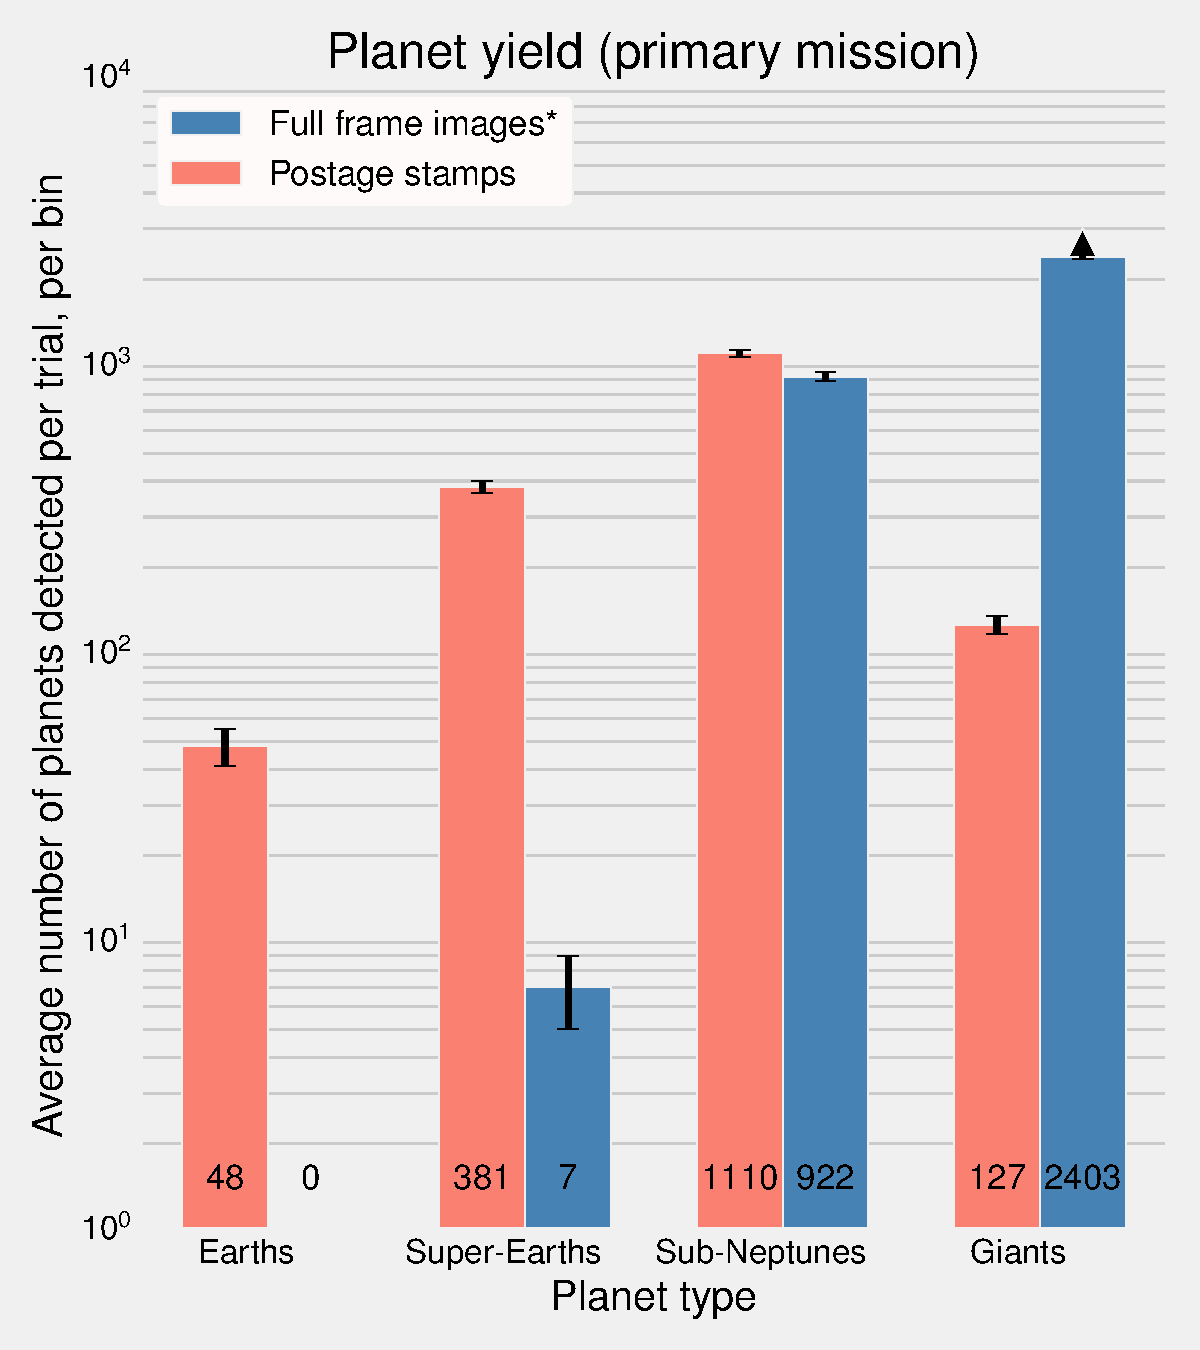
\includegraphics[width=\textwidth]{figures/160729_pm0_shemi_nhemi_nhemi_t20-pri-yield.pdf}
	\caption{Mean numbers of planets detected in \tesss primary mission (error bars are from Poisson fluctuations and do not account for systematic uncertainty). 
		In postage stamp detections, the number of Earths ($R_p < 1.25R_\oplus$), super-Earths ($1.25R_\oplus \le R_p < 2R_\oplus$), sub-Neptunes ($2R_\oplus \le R_p < 4R_\oplus$) and giants ($R_p > 4R_\oplus$) is comparable to those quoted in \protect\citet{Sullivan_2015}, despite modifications to our target selection procedure (Sec.~\protect\ref{sec:selection_criteria}).
		Our full frame images detections in are complete for $R < 4R_\oplus$, and incomplete for giant planets. 
		Here we disagree, by for instance two orders of magnitude in the super-Earth bin, with~\protect\citet{Sullivan_2015} (see text). }
	\label{fig:primary_planet_yield}
\end{marginfigure}
We first examine our results for just the first two years of \tesss observing, before presenting an analysis of our detected planet populations from a single extended mission (Sec.~\ref{sec:results_from_nhemi_extended_mission}) and all six of our proposed extended missions (Sec.~\ref{sec:results_from_all_extended_missions}).
Here we highlight commonalities and differences between~\citetalias{Sullivan_2015} and this work.

\paragraph{Detected planet yield}
The first point of comparison is the detected planet yield from our simulation, shown in Fig.~\ref{fig:primary_planet_yield}.
The number of Earths, super-Earths, sub-Neptunes and giants we detect in postage stamps agrees with the numbers quoted in~\citetalias{Sullivan_2015}, despite our modified target selection procedure.
Other changes to our simulation's inputs, for instance using an as-built model of \tesss PSF informed by laboratory tests (courtesy Deborah Woods) rather than the idealized PSF described in Sec6.1 of~\citetalias{Sullivan_2015}, also had little impact on this final result.

However, our yields from full frame images differ markedly from those quoted in Fig. 18 of~\citetalias{Sullivan_2015}.
We agree with~\citetalias{Sullivan_2015} that no Earths are detected in the full frame images.
However, we detect only $\sim10$ super-Earths by observing the $200,001\mathrm{^{st}}$ to $4,000,000\mathrm{^{th}}$ \texttt{Merit}-ranked stars at 30 minute cadence.
This is two orders of magnitude less than the $\sim1000$ super-Earth detections claimed from FFIs in~\citetalias{Sullivan_2015}.
There is also a small discrepancy in FFI-detected sub-Neptunes, for which we claim detection of $\sim1000$, while~\citetalias{Sullivan_2015} claims $\sim2000$.

We empirically verified that our full frame image detections are complete for $R < 4R_\oplus$ by changing the number of stars observed at 30-minute cadence and seeing that the number of detected planets with radii less than Neptune did not change.
%In this context,~\citetalias{Sullivan_2015}'s claim of detecting $1000$ super-Earths in \tesss full-frame images must be false.
We do not understand the origin of the difference between our method and~\citetalias{Sullivan_2015}'s, but note that our results are in much better agreement with order-of-magnitude analytic arguments for \tesss expected planet yield.
Assuming an exponentially distributed stellar population in the galaxy and computing limiting magnitude thresholds,~\citet{winn_searchable_2013} predicted detections of $600-6000$ Neptunes, $24-300$ super-Earths, and $1-10$ Earth-sized planets, where the lower bounds correspond to planets detected with $\mathrm{SNR}>10$, and the upper bounds for $\mathrm{SNR}>7$.
~\citetalias{Sullivan_2015}'s prediction of a total of $1500$ detected super-Earths is a factor of 5 larger than these analytic estimates, while ours is in rough (< factor of 2) agreement.

We also present the following plausibility argument for our yields vs. those of~\citetalias{Sullivan_2015}:
consider the two adjacent bins of the relevant histogram, where one bin has width $0.75R_\oplus$ and 1400 planets fall within it, and the other has width $2R_\oplus$ and 3000 planets fall in it if we believe~\citetalias{Sullivan_2015}, and 400 and 2000 do if we believe our own work.
Letting `rate' mean the number per bin width, this means that ratio of the rates of detected super-Earths to sub-Neptunes for~\citetalias{Sullivan_2015}'s case is $(1400/0.75R_\oplus)/(3000/2R_\oplus)=1.25$, and for our case it is $(400/0.75_\oplus)/(2000/2R_\oplus)=0.53$.
The actual \textit{input} ratio for these rates (cf.~\citetalias{Sullivan_2015}, Fig 8) is about $2$ for $T_\mathrm{eff}<4000$K hosts and $1.5$ for $T_\mathrm{eff}>4000$K hosts.
In the top $4\times10^6$ merit ranked stars from TRILEGAL (those that we empirically saw give all $R_p<4R_\oplus$ planets), 31\% of them have $T_\mathrm{eff} < 4000\mathrm{K}$.
Thus the weighted input ratio is roughly $2\times0.31 + 1.5\times0.69=1.66$. %perhaps slightly more given that we detect the biggest fraction of our planets around M dwarfs\footnote{It turns out below this only helps our case.}.
\citetalias{Sullivan_2015}'s result is that the detection bias for super-Earths (typically $R_p=1.5R_\oplus$) versus sub-Neptunes (typically $R_p=3R_\oplus$) is so slight that actually observing leads to a relative loss of $1.66/1.25=1.3\times$ fewer super-Earths than sub-Neptunes.
Our result is that it's $1.66/0.53=3.1\times$ fewer.
A naive expectation would have us believe that it's 4$\times$ fewer, given that $\delta\propto R_p^2$.
This means that~\citetalias{Sullivan_2015}'s results imply a detection efficiency biased sub-linearly in $R_p$, whilst ours implies a bias between linear and quadratic in $R_p$.

% Also, Peter's data from plat10r.fits, May 4 2015, agree with my results. I never was able to find the data with his FFI numbers...
\paragraph{Properties of planets detected in primary mission} 
We show the population properties of planets detected from postage stamps and full frame images in the primary mission in Figs.~\ref{fig:radius_vs_period_nhemi} and~\ref{fig:imag_vs_teff_nhemi}.
We agree with~\citetalias{Sullivan_2015} for all major postage stamp properties (apparent magnitude $I_C$, planet radius $R_p$, orbital period $P$, and insolation $S$), while, as discussed above, differing in full frame image yields.
For instance, the dearth of $P<5$ day Neptune-radius planets in Fig.~\ref{fig:radius_vs_period_nhemi} was observed by \textit{Kepler}~\citep{mazeh_dearth_2016}, and thus it is present in our input occurrence rates, rather than being an observational bias. 
It was also seen in~\citetalias{Sullivan_2015}.

The differences between planets detected in postage stamps vs. in full frame images follow our expectation from our \texttt{Merit} statistic. 
Namely, Fig.~\ref{fig:imag_vs_teff_nhemi} shows that at a fixed brightness, full frame image detections tend to occur at larger stellar effective temperature (and thus stellar radius).
At a fixed host star radius, postage stamp detections occur around brighter stars.

\paragraph{Impact of earth and moon crossings on primary mission's detected planet yield}
We drop the most fields for Camera 1 in Year 2 of the primary (4 of 13 `observing sectors', see Table~\ref{tab:dropped_fields} and Fig.~\ref{fig:earth_moon_primary}).
This reduces the number of planet detections near the ecliptic at the beginning of Year 2, in some fields to zero.
This is visible in the orange points of Fig.~\ref{fig:skymap_nhemi}.
In the primary mission \tess detects $\sim20$ planets with $R_p<4R_\oplus$ from both 2 minute and 30 minute data in each $24^\circ\times24^\circ$ camera field nearest to the ecliptic (where each field is observed for 2 \tess orbits).
As implemented in our simulation, Earth and Moon crossings result in fields simply not being observed, so in these cases planets orbiting stars in these fields are never detected.
Considering only the primary mission, we would naively expect that dropping a total of 9 fields over the two years (again, see Table~\ref{tab:dropped_fields}) would result in a loss of $\sim9\times20=180$ planets.
This agrees with what our simulations actually give: running them without accounting for Earth and Moon losses returns a mean of 2678 detected planets with $R_p<4R_\oplus$, while running them with Earth and Moon crossings gives a mean of 2482 such planets (a loss of 196 planets, or $7\%$ of the sub-Neptune yield).
% data from 160708-t50 and 160729-t20. Slightly apples to oranges because of number of trials difference, but makes the point. 